\documentclass[../main/main.tex]{subfiles}

\newdate{date}{11}{10}{2019}

\begin{document}

\section{Grancanonical potential}
\marginpar{ \textbf{Lecture 2.} \\  \displaydate{date}. \\ Compiled:  \today.}
The two intensive variables to became indipendent are \emph{T} and \( \mu  \). The corresponding Legendre transform is
\begin{equation}
  \Omega = U -T S - \sum_{i=1}^{r} \mu _i N _i = A - \sum_{i=1}^{r}  \mu _i N _ i
  \label{eq:}
\end{equation}
Differentiating this relation we obtain:
\begin{equation}
\begin{split}
\dd[]{\Omega }   &=  \dd[]{U} - S \dd[]{T} - T \dd[]{S} - \sum_{ij}^{} \dd[]{\mu _j} N_j - \sum_{i=1}^{r} \mu _i \dd[]{N_i}           \\
& = (\delta Q - T \dd[]{S}) - \delta W - S \dd[]{T} - \sum_{j=1}^{r} \dd[]{\mu _j} N_j - \sum_{j=1}^{r} \mu _j \dd[]{N_j}
\end{split}
  \label{eq:}
\end{equation}
Hence, \( \Omega = \Omega (T,P,{\mu _j}) \).
Internal energy $U$ and entropy $S$ are homogeneus function of the first order. A consequence of this fact is the relation called \textbf{Euler equation}:
\begin{equation}
  U = T S - P V + \sum_{j}^{} \mu _j N_j
  \label{eq:}
\end{equation}
Instead, the \textbf{Maxwell relations} are relations between the mixed derivatives of the thermodynamic potentials. They can be obtained from the expressions of \( \dd[]{U},\dd[]{H} ,\dd[]{A}, \dd[]{G}    \)  and \( \dd[]{\Omega }  \) and from the Schwarz theorem on mixed partial derivatives.
Due to Schwarz theorem, if a thermodynamic potential depends on \( t+1 \) variables there will be \( \frac{t(t+1)}{2} \)  indipendent mixed derivatives.
\begin{example}[Internal energy]
\begin{equation}
  \dd[]{U} = T \dd[]{S} - P \dd[]{V} + \mu \dd[]{N}
  \label{eq:2_1}
\end{equation}
where \( T = \qty(\pdv{U}{S} )_{V,N}  \) and  \( -P = \qty(\pdv{U}{V} )_{S,N}  \). It implies that
\begin{equation*}
        \pdv{U}{V}{S} = \qty(\pdv{T}{V} )_{S,N} \underset{\substack{ \text{from } \\  \text{Schwarz inequality} } }{=} -\qty(\pdv{P}{S} )_{V,N}
\end{equation*}
therefore, we have the \emph{1° Maxwell relation} :
\begin{equation*}
  \qty(\pdv{T}{V} )_{S,N} = -\qty(\pdv{P}{S} )_{V,N}
\end{equation*}
All the \emph{3 Maxweel relations} obtained by the differential \eqref{eq:2_1}
with \( t=2 \), for which we have \( t+1=3 \) and \( \frac{t(t+1)}{2}=3 \) (\( [S,V,N] \) ), are

\begin{subequations}
\begin{align}
  (S,V) &:& \qty(\pdv{T}{V} )_{S,N} =& - \qty(\pdv{P}{S} )_{V,N} & \\
  (S,N) &:& \qty(\pdv{T}{N} )_{V,S} =& \qty(\pdv{\mu }{S} )_{V,N} &\\
  (V,N) &:& -\qty(\pdv{P}{N} )_{S,V} =& \qty(\pdv{\mu }{V} )_{S,N} &
 \end{align}
\label{}
\end{subequations}
\end{example}

\begin{example}[Helmholz \( A=A(T,V,N) \)]
\begin{equation}
  \dd[]{A} = - S \dd[]{T} - P \dd[]{V} + \mu \dd[]{N}
\end{equation}
In this case the \emph{3 Maxweel relations} (\( [T,V,N] \) ) are
\begin{subequations}
\begin{align}
  (T,V) &:& \qty(\pdv{S}{V} )_{T,N} =&  \qty(\pdv{P}{T} )_{V,N} & \\
  (T,N) &:& -\qty(\pdv{S}{N} )_{T,V} =& \qty(\pdv{\mu }{T} )_{V,N} &\\
  (V,N) &:& -\qty(\pdv{P}{N} )_{V,T} =& \qty(\pdv{\mu }{V} )_{T,N} &
 \end{align}
\label{}
\end{subequations}
\end{example}
\begin{example}[Gibbs \( G=G(T,P,N) \) ]
  \begin{equation}
    \dd[]{G} = - S \dd[]{T} - V \dd[]{P} + \mu \dd[]{N}
  \end{equation}
  In this case the \emph{3 Maxweel relations} (\( [T,P,N] \) ) are
  \begin{subequations}
  \begin{align}
    (T,P) &:& -\qty(\pdv{S}{P} )_{T,N} =&  \qty(\pdv{V}{T} )_{P,N} & \\
    (T,N) &:& -\qty(\pdv{S}{N} )_{T,P} =& \qty(\pdv{\mu }{T} )_{P,N} &\\
    (P,N) &:& \qty(\pdv{V}{N} )_{P,T} =& \qty(\pdv{\mu }{P} )_{T,N} &
   \end{align}
  \label{}
  \end{subequations}
\end{example}

\section{Response functions}
Aim of most experiments is to measure the response of a thermodynamic system write respect to controlled variatious of thermodynamic variables. In fact, any osservation is just the pertubation of a system and looking for the response.
A list of the commonly used response functions is the following:
\begin{itemize}
\item \emph{Thermal expansion coefficient at constant pressure}.
\begin{equation}
  \alpha _P \equiv \frac{1}{V} \qty(\pdv{V}{T} )_{P,N}
  \label{eq:}
\end{equation}
\item \emph{Molar heat capacity at constant pressure}.
\begin{equation}
  c_P = \qty(\frac{\delta Q}{\dd[]{T} } )_P = T \qty(\pdv{S}{T} )_P \underset{-S=\qty(\pdv{G}{T} )_P }{=}  - T \qty(\pdv[2]{G}{T} )_P
  \label{eq:}
\end{equation}
\item \emph{Adiabatic compressibility}.
\begin{equation}
  k_S = -\frac{1}{V} \qty(\pdv{V}{P} )_{S,N} \underset{V=\qty(\pdv{H}{P} )_{S,N} }{=} - \frac{1}{V} \qty(\pdv[2]{H}{P} )_{S,N}
    \label{eq:}
\end{equation}
\item \emph{Isothermal compressibility} .
\begin{equation}
  k_T = -\frac{1}{V} \qty(\pdv{V}{P} )_{T,N} \underset{V=\qty(\pdv{G}{P} )_{T,N} }{=} - \frac{1}{V} \qty(\pdv[2]{G}{P} )_{T,N}
  \label{eq:}
\end{equation}
\begin{remark}
Remember that \( k_T \) it is the second derivative of the Gibbs potential write respect to pressure.
\end{remark}
\item \emph{Specific heat at constant volume}. Consider a quasi static transformation.
\begin{equation}
  c_V =  \qty(\frac{\delta Q}{\dd[]{T} } )_{V,N} = T \qty(\pdv{S}{T} )_{V,N}
      = \qty( \frac{\partial{(-\partial{A}/\partial{T} )_{V,N}} }{\partial{T} })_{V,N}
      = - T \qty(\pdv[2]{A}{T} )_{V,N}
  \label{eq:}
\end{equation}
\item \emph{Magnetic suscettibility (d=1)} for a magnetic system \( (\va{M},\va{H},T  ) \).
\begin{equation}
  \chi_T = \qty(\pdv{M}{H} )_T \underset{M = -\eval{\pdv{G}{H}}_T }{=}  - \qty(\pdv[2]{G}{H} )_T
  \label{eq:}
\end{equation}
More generals, \( \va{M},\va{H}   \) we have
\begin{equation}
  \chi _{\alpha \beta } = \qty(\pdv{M_ \alpha }{H_ \beta } )_T , M_ \alpha = -\eval{\pdv{G}{H_ \alpha }}_T \Rightarrow \chi _{\alpha \beta } = \eval{\pdv{G}{H_ \beta }{H_ \alpha }}_T
  \label{eq:}
\end{equation}

\end{itemize}
Note that the response functions, when used with the Maxwell relations, allow to express observables usually inaccessible to experiments with measurable quantitities.
\begin{example}[The Maxwell relation]
  \begin{equation*}
    \qty(\pdv{S}{P} )_{T,N} = - \qty(\pdv{V}{T} )_{P,N}
  \end{equation*}
  obtained from
  \begin{equation*}
\dd[]{G} = - S \dd[]{T} + V \dd[]{P}
  \end{equation*}
and the response function \( \alpha _P \) permit to write
\begin{equation}
  \underbrace{\qty(\pdv{S}{P} )_{T,N}}_{\substack{ \text{inaccessible} \\  \text{to experiments} } }  = \underbrace{- V \alpha _P}_{\text{measurable}}
  \label{eq:}
\end{equation}
\end{example}
\begin{example}
Let us start with the Maxwell relation
\begin{equation*}
  \qty(\pdv{S}{V} )_{T,N} =  \qty(\pdv{P}{T} )_{V,N}
\end{equation*}
obtained from
\begin{equation*}
    \dd[]{A} = - S \dd[]{T} - P \dd[]{V} + \mu \dd[]{N}
\end{equation*}
From some property of multi-variable differential calculus one has the \textbf{triple product rule}:
\begin{equation}
    \qty(\pdv{P}{T} )_{V,N}  \qty(\pdv{V}{P} )_{T,N}   \qty(\pdv{T}{V} )_{P,N} =-1
  \label{eq:}
\end{equation}
Hence
\begin{equation}
\begin{split}
    \qty(\pdv{P}{T} )_{V,N} &= \frac{-1}{ \qty(\pdv{V}{P} )_{T,N}   \qty(\pdv{T}{V} )_{P,N} }  = - \frac{  \qty(\pdv{V}{T} )_{P,N} }{   \qty(\pdv{V}{P} )_{T,N} } \\
    &= \frac{-V \alpha _P}{-V k_T} = \frac{\alpha _P}{k _T}
\end{split}
  \label{eq:}
\end{equation}
\end{example}

\section{Response functions and thermodynamic stability}
Now, we analyze the concept of \textbf{thermal stability}. If one injects heat in a system either at constant volume or at constant pressure, its temperature will inevitably increase
\begin{equation}
  \begin{cases}
   c_V \equiv \qty(\frac{\delta Q}{\dd[]{T} })_V \ge 0  \\
   c_P \equiv \qty(\frac{\delta Q}{\dd[]{T} })_P \ge 0
  \end{cases}
\label{eq:}
\end{equation}
\begin{remark}
The thermal capacities are \emph{non-negative functions}!
\end{remark}
It is useful also the concept of \textbf{mechanical stability}. If one compress a system by keeping \emph{T} constant, we would expect that it shrinks
\begin{equation}
  k_T = - \frac{1}{V} \qty(\pdv{V}{P} )_T \ge 0
  \label{eq:}
\end{equation}
Similar considerations for a magnetic system, gives
\begin{equation}
  c_H \ge 0, \quad c_M \ge 0, \quad \chi_M \ge 0
  \label{eq:}
\end{equation}
\begin{remark}
In diamangetic systems \( \chi_M \) can also be negative.
\end{remark}

\begin{exercise}
By using Maxwell relations show that
\begin{subequations}
\begin{align}
  c_P - c_V &= \frac{T V \alpha ^2}{k_T} = \frac{1}{V k_T} T \qty(\pdv{V}{T} )_P^2 \\
  c_H - c_M &= \frac{T}{\chi _T} \qty(\pdv{M}{T} )_H^2
\end{align}
\label{}
\end{subequations}
\end{exercise}
\noindent A consequence is that since the right hand terms are non negative it follows that
\begin{equation}
  \begin{cases}
   c_P \ge c_V \ge 0  \\
   c_H \ge c_M \ge 0
  \end{cases}
\label{eq:}
\end{equation}

For reasuming, we have seen the thermodynamic of a phase, where the equilibrium state can be described by the maximum of the entropy. If we have a given phase, we can look for the Gibbs function. If we have more phases, we want to change between these phases.















\chapter{Equilibrium phases and thermodynamics of phase transitions}

\section{Equilibrium phases as minima of Gibbs free energy}

Equilibrium states are given by \emph{maxima} of the entropy and \emph{minima} of internal energy, or by \emph{minima} of thermodynamics potentials such as \emph{A} and \emph{G}.
Let us consider for example the Gibbs potential per particle of a fluid system
\begin{equation}
  \frac{G}{N} \equiv g = g (T,P)
  \label{eq:}
\end{equation}
  that depends on two intensive variables \emph{T} and \emph{P} and is not anymore a function of \emph{N} because we have divided for \emph{N}.
  Let us define \( \alpha  \) the phase of a one-component system (say \( \alpha = \) gas or liquid ). Therfore, the thermodynamic properties are described by surfaces of function \( g_\alpha (T,P) \) and for all equilibrium phase we have a surface on the space (T,P,g). For each value of \emph{T} and \emph{P} the thermodynamically stable phase is the one for which \( g_ \alpha (T,P) \) is minimum.

\section{First order phase transition and phase coexistence}

Consider the surface \( g_ \alpha  \) and \( g_ \beta  \), we are looking for the lower one (Figure \ref{fig:2_1}) and there is a moment in which they coexist.
The coexistence line is the projection on the \emph{(T,P)} plane of the intersection between different surfaces, so the \textbf{coexistence condition} is:
\begin{equation}
g_ \alpha(T,P) = g_ \beta(T,P)
  \label{eq:}
\end{equation}



\begin{figure}[h!]
\centering


\tikzset{every picture/.style={line width=0.75pt}} %set default line width to 0.75pt

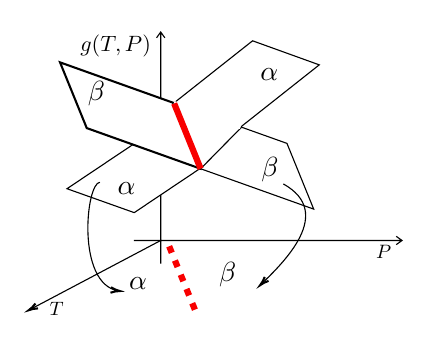
\begin{tikzpicture}[x=0.75pt,y=0.75pt,yscale=-0.4,xscale=0.4]
%uncomment if require: \path (0,440); %set diagram left start at 0, and has height of 440

%Shape: Axis 2D [id:dp40801434027932515]
\draw  (212,260.1) -- (535,260.1)(244.3,9) -- (244.3,288) (528,255.1) -- (535,260.1) -- (528,265.1) (239.3,16) -- (244.3,9) -- (249.3,16)  ;
%Straight Lines [id:da5508882643216593]
\draw    (244.3,260.1) -- (87.07,343.17) ;
\draw [shift={(85.3,344.1)}, rotate = 332.15] [color={rgb, 255:red, 0; green, 0; blue, 0 }  ][line width=0.75]    (10.93,-3.29) .. controls (6.95,-1.4) and (3.31,-0.3) .. (0,0) .. controls (3.31,0.3) and (6.95,1.4) .. (10.93,3.29)   ;

%Shape: Parallelogram [id:dp6573265862021008]
\draw  [fill={rgb, 255:red, 255; green, 255; blue, 255 }  ,fill opacity=1 ] (211.09,144.37) -- (292.08,173.17) -- (212.41,226.56) -- (131.42,197.75) -- cycle ;
%Shape: Parallelogram [id:dp550630493685483]
\draw  [fill={rgb, 255:red, 255; green, 255; blue, 255 }  ,fill opacity=1 ] (396.38,143.17) -- (428.57,222.33) -- (292.38,173.7) -- (260.18,94.54) -- cycle ;
%Shape: Parallelogram [id:dp7252967331246472]
\draw  [fill={rgb, 255:red, 255; green, 255; blue, 255 }  ,fill opacity=1 ][line width=0.75]  (259.21,94.18) -- (291.41,173.35) -- (155.21,124.72) -- (123.02,45.55) -- cycle ;
%Shape: Parallelogram [id:dp3266181656966768]
\draw  [color={rgb, 255:red, 0; green, 0; blue, 0 }  ,draw opacity=1 ][fill={rgb, 255:red, 255; green, 255; blue, 255 }  ,fill opacity=1 ] (340.5,123.52) -- (260.18,94.54) -- (354.95,19.59) -- (435.26,48.57) -- cycle ;
%Straight Lines [id:da6729139269661627]
\draw    (341.47,123.88) -- (292.38,173.7) ;


%Straight Lines [id:da11695782732739401]
\draw [color={rgb, 255:red, 255; green, 255; blue, 255 }  ,draw opacity=1 ][fill={rgb, 255:red, 255; green, 255; blue, 255 }  ,fill opacity=1 ][line width=1.5]    (260.18,94.54) -- (340.5,123.52) ;


%Straight Lines [id:da3638306026418753]
\draw [color={rgb, 255:red, 248; green, 0; blue, 0 }  ,draw opacity=1 ][line width=2.25]    (260.48,95.07) -- (292.38,173.7) ;


%Straight Lines [id:da014936569885654949]
\draw [color={rgb, 255:red, 248; green, 0; blue, 0 }  ,draw opacity=1 ][line width=2.25]  [dash pattern={on 2.53pt off 3.02pt}]  (254.48,267.07) -- (286.38,345.7) ;


%Curve Lines [id:da7725903059840692]
\draw    (171,190) .. controls (154.17,190.99) and (142.24,312.53) .. (193.43,320.78) ;
\draw [shift={(195,321)}, rotate = 186.46] [color={rgb, 255:red, 0; green, 0; blue, 0 }  ][line width=0.75]    (10.93,-3.29) .. controls (6.95,-1.4) and (3.31,-0.3) .. (0,0) .. controls (3.31,0.3) and (6.95,1.4) .. (10.93,3.29)   ;

%Curve Lines [id:da5672055830816675]
\draw    (392,192) .. controls (454.06,226.48) and (392.89,286.18) .. (365.24,312.81) ;
\draw [shift={(364,314)}, rotate = 316.08000000000004] [color={rgb, 255:red, 0; green, 0; blue, 0 }  ][line width=0.75]    (10.93,-3.29) .. controls (6.95,-1.4) and (3.31,-0.3) .. (0,0) .. controls (3.31,0.3) and (6.95,1.4) .. (10.93,3.29)   ;


% Text Node
\draw (203,198) node   {$\alpha $};
% Text Node
\draw (375,60) node   {$\alpha $};
% Text Node
\draw (167,83.7) node   {$\beta $};
% Text Node
\draw (376,174.7) node   {$\beta $};
% Text Node
\draw (119,343) node [scale = 0.7]  {$T$};
% Text Node
\draw (513,274) node  [scale = 0.7] {$P$};
% Text Node
\draw (217,312) node   {$\alpha $};
% Text Node
\draw (325,300.7) node   {$\beta $};
% Text Node
\draw (190,26) node [scale = 0.8]  {$g( T,P)$};

\end{tikzpicture}

\caption{\label{fig:2_1} Description.}
\end{figure}

To fix the ideas, let us choose a given value of pressure \( P = P^* \) and study the behaviour of \( g(T,P^*) \) as a function of \emph{T} when we go from solid to gas (Figure \ref{fig:2_2}).
At the triple point \( g_{\text{solid}}(T_ a, P^*) = g_{\text{liq}}(T_a) \) and \( g_{\text{liq}}(T_b) = g_{\text{gas}}(T_b , P^*) \) (see Figure \ref{fig:2_3} ).
Note also that:
\begin{itemize}
\item At the coexistence points \emph{a} and \emph{b} of the two phases, one has \( g_ \alpha (T) = g_ \beta (T) \).
\item \( g(T) \) is a continuous function of \emph{T}.
\item Note that, \( S= -\qty(\pdv{G}{T} )_V  \)  and \( c_P = - T \qty(\pdv[2]{G}{T}) > 0 \). This implies that \( g(T) \) is concave in \emph{T} at fixed \emph{P}.
\end{itemize}



\begin{figure}[h!]
\begin{minipage}[c]{0.5\linewidth}
\centering
\subfloat[][Description]{




\tikzset{every picture/.style={line width=0.75pt}} %set default line width to 0.75pt

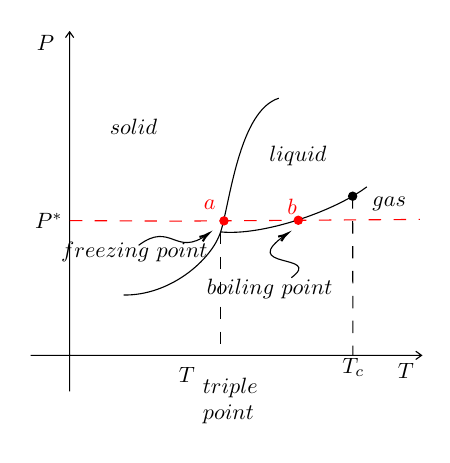
\begin{tikzpicture}[x=0.75pt,y=0.75pt,yscale=-0.4,xscale=0.4]
%uncomment if require: \path (0,433); %set diagram left start at 0, and has height of 433

%Shape: Axis 2D [id:dp34042133393206886]
\draw  (72,390.7) -- (543,390.7)(119.1,1) -- (119.1,434) (536,385.7) -- (543,390.7) -- (536,395.7) (114.1,8) -- (119.1,1) -- (124.1,8)  ;
%Curve Lines [id:da2649058921866929]
\draw    (184,318) .. controls (240,319) and (290,276) .. (301,242) .. controls (312,208) and (323,96) .. (371,81) ;


%Curve Lines [id:da19336772925785306]
\draw    (301,242) .. controls (351,247) and (437.06,217.73) .. (477.06,187.73) ;


%Straight Lines [id:da1379576233427211]
\draw  [dash pattern={on 4.5pt off 4.5pt}]  (301,242) -- (301,390) ;


%Straight Lines [id:da6702336744569144]
\draw  [dash pattern={on 4.5pt off 4.5pt}]  (460,199) -- (460.35,390.47) ;


%Straight Lines [id:da9070120311351494]
\draw [color={rgb, 255:red, 255; green, 0; blue, 0 }  ,draw opacity=1 ] [dash pattern={on 4.5pt off 4.5pt}]  (119.33,228.35) -- (248,229) -- (541.11,226.96) ;


%Shape: Circle [id:dp6233075621783745]
\draw  [color={rgb, 255:red, 255; green, 0; blue, 0 }  ,draw opacity=1 ][fill={rgb, 255:red, 255; green, 0; blue, 0 }  ,fill opacity=1 ] (300.09,228.71) .. controls (300.09,225.98) and (302.31,223.76) .. (305.05,223.76) .. controls (307.78,223.76) and (310,225.98) .. (310,228.71) .. controls (310,231.45) and (307.78,233.67) .. (305.05,233.67) .. controls (302.31,233.67) and (300.09,231.45) .. (300.09,228.71) -- cycle ;
%Shape: Circle [id:dp768993062031393]
\draw  [color={rgb, 255:red, 255; green, 0; blue, 0 }  ,draw opacity=1 ][fill={rgb, 255:red, 255; green, 0; blue, 0 }  ,fill opacity=1 ] (389.6,227.98) .. controls (389.6,225.24) and (391.82,223.03) .. (394.55,223.03) .. controls (397.29,223.03) and (399.51,225.24) .. (399.51,227.98) .. controls (399.51,230.72) and (397.29,232.93) .. (394.55,232.93) .. controls (391.82,232.93) and (389.6,230.72) .. (389.6,227.98) -- cycle ;
%Curve Lines [id:da897292552339868]
\draw    (202.21,258.16) .. controls (241.81,228.46) and (246.13,273.25) .. (285.02,245.04) ;
\draw [shift={(286.21,244.16)}, rotate = 503.13] [color={rgb, 255:red, 0; green, 0; blue, 0 }  ][line width=0.75]    (10.93,-3.29) .. controls (6.95,-1.4) and (3.31,-0.3) .. (0,0) .. controls (3.31,0.3) and (6.95,1.4) .. (10.93,3.29)   ;

%Curve Lines [id:da43687585409049334]
\draw    (386.21,297.16) .. controls (426.01,267.31) and (318.3,287.95) .. (380.27,244.82) ;
\draw [shift={(381.21,244.16)}, rotate = 505.49] [color={rgb, 255:red, 0; green, 0; blue, 0 }  ][line width=0.75]    (10.93,-3.29) .. controls (6.95,-1.4) and (3.31,-0.3) .. (0,0) .. controls (3.31,0.3) and (6.95,1.4) .. (10.93,3.29)   ;

%Shape: Circle [id:dp07400034471483774]
\draw  [color={rgb, 255:red, 0; green, 0; blue, 0 }  ,draw opacity=1 ][fill={rgb, 255:red, 0; green, 0; blue, 0 }  ,fill opacity=1 ] (455.05,199) .. controls (455.05,196.26) and (457.26,194.05) .. (460,194.05) .. controls (462.74,194.05) and (464.95,196.26) .. (464.95,199) .. controls (464.95,201.74) and (462.74,203.95) .. (460,203.95) .. controls (457.26,203.95) and (455.05,201.74) .. (455.05,199) -- cycle ;

% Text Node
\draw (196,116) node  [scale=0.8] {$solid$};
% Text Node
\draw (394,150) node  [scale=0.8] {$liquid$};
% Text Node
\draw (504,208) node   [scale=0.8]{$gas$};
% Text Node
\draw (94,228.73) node [scale=0.8]  {$P^{*}$};
% Text Node
\draw (288,209) node [scale=0.8][color={rgb, 255:red, 255; green, 0; blue, 0 }  ,opacity=1 ]  {$a$};
% Text Node
\draw (387,212) node [scale=0.8][color={rgb, 255:red, 255; green, 0; blue, 0 }  ,opacity=1 ]  {$b$};
% Text Node
\draw (197,266.16) node  [scale=0.8] {$freezing\ point$};
% Text Node
\draw (360,311.16) node  [scale=0.8] {$boiling\ point$};
% Text Node
\draw (310,441.16) node  [scale=0.8] {$T_{ \begin{array}{l}
triple\ \\
point
\end{array}}$};
% Text Node
\draw (461,405.16) node [scale=0.8]  {$T_{c}$};
% Text Node
\draw (90,14) node  [scale=0.8] {$P$};
% Text Node
\draw (524,409) node  [scale=0.8] {$T$};


\end{tikzpicture}


    \label{fig:2_2} }
\end{minipage}
\begin{minipage}[]{0.5\linewidth}
\centering
\subfloat[][Description]{


\tikzset{every picture/.style={line width=0.75pt}} %set default line width to 0.75pt

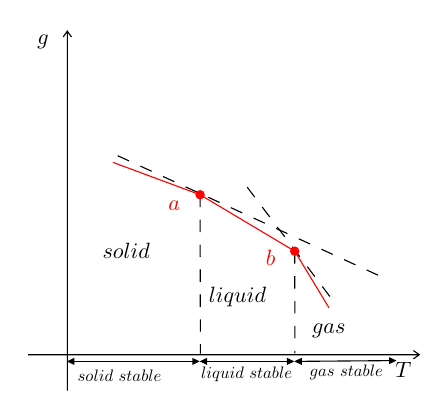
\begin{tikzpicture}[x=0.75pt,y=0.75pt,yscale=-0.4,xscale=0.4]
%uncomment if require: \path (0,433); %set diagram left start at 0, and has height of 433

%Shape: Axis 2D [id:dp34042133393206886]
\draw  (72,390.7) -- (543,390.7)(119.1,1) -- (119.1,434) (536,385.7) -- (543,390.7) -- (536,395.7) (114.1,8) -- (119.1,1) -- (124.1,8)  ;
%Straight Lines [id:da1379576233427211]
\draw  [dash pattern={on 4.5pt off 4.5pt}]  (393,266) -- (393.24,389.13) ;


%Straight Lines [id:da6702336744569144]
\draw  [dash pattern={on 4.5pt off 4.5pt}]  (279,198) -- (279.35,389.47) ;


%Straight Lines [id:da4803241471694518]
\draw [color={rgb, 255:red, 255; green, 0; blue, 0 }  ,draw opacity=1 ]   (174,159) -- (279,198) -- (393,266) -- (434.24,334.13) ;


%Straight Lines [id:da30479529109521597]
\draw  [dash pattern={on 4.5pt off 4.5pt}]  (179.78,151) -- (493.37,294.92) ;


%Shape: Circle [id:dp5413533969874785]
\draw  [color={rgb, 255:red, 255; green, 0; blue, 0 }  ,draw opacity=1 ][fill={rgb, 255:red, 255; green, 0; blue, 0 }  ,fill opacity=1 ] (274.05,198) .. controls (274.05,195.26) and (276.26,193.05) .. (279,193.05) .. controls (281.74,193.05) and (283.95,195.26) .. (283.95,198) .. controls (283.95,200.74) and (281.74,202.95) .. (279,202.95) .. controls (276.26,202.95) and (274.05,200.74) .. (274.05,198) -- cycle ;
%Straight Lines [id:da540096881916741]
\draw  [dash pattern={on 4.5pt off 4.5pt}]  (335.78,188.92) -- (443.22,331) ;


%Shape: Circle [id:dp33029146551714716]
\draw  [color={rgb, 255:red, 255; green, 0; blue, 0 }  ,draw opacity=1 ][fill={rgb, 255:red, 255; green, 0; blue, 0 }  ,fill opacity=1 ] (388.05,266) .. controls (388.05,263.26) and (390.26,261.05) .. (393,261.05) .. controls (395.74,261.05) and (397.95,263.26) .. (397.95,266) .. controls (397.95,268.74) and (395.74,270.95) .. (393,270.95) .. controls (390.26,270.95) and (388.05,268.74) .. (388.05,266) -- cycle ;
%Straight Lines [id:da5141015065570389]
\draw    (120.56,398.75) -- (276.56,398.75) ;
\draw [shift={(278.56,398.75)}, rotate = 180] [fill={rgb, 255:red, 0; green, 0; blue, 0 }  ][line width=0.75]  [draw opacity=0] (8.93,-4.29) -- (0,0) -- (8.93,4.29) -- cycle    ;
\draw [shift={(118.56,398.75)}, rotate = 0] [fill={rgb, 255:red, 0; green, 0; blue, 0 }  ][line width=0.75]  [draw opacity=0] (8.93,-4.29) -- (0,0) -- (8.93,4.29) -- cycle    ;
%Straight Lines [id:da18116836165751382]
\draw    (280.56,398.75) -- (390.56,398.75) ;
\draw [shift={(392.56,398.75)}, rotate = 180] [fill={rgb, 255:red, 0; green, 0; blue, 0 }  ][line width=0.75]  [draw opacity=0] (8.93,-4.29) -- (0,0) -- (8.93,4.29) -- cycle    ;
\draw [shift={(278.56,398.75)}, rotate = 0] [fill={rgb, 255:red, 0; green, 0; blue, 0 }  ][line width=0.75]  [draw opacity=0] (8.93,-4.29) -- (0,0) -- (8.93,4.29) -- cycle    ;
%Straight Lines [id:da9621936586212539]
\draw    (394.56,398.74) -- (513.56,397.77) ;
\draw [shift={(515.56,397.75)}, rotate = 539.53] [fill={rgb, 255:red, 0; green, 0; blue, 0 }  ][line width=0.75]  [draw opacity=0] (8.93,-4.29) -- (0,0) -- (8.93,4.29) -- cycle    ;
\draw [shift={(392.56,398.75)}, rotate = 359.53] [fill={rgb, 255:red, 0; green, 0; blue, 0 }  ][line width=0.75]  [draw opacity=0] (8.93,-4.29) -- (0,0) -- (8.93,4.29) -- cycle    ;

% Text Node
\draw (190,265) node [scale=0.8]  {$solid$};
% Text Node
\draw (324,321) node [scale=0.8]  {$liquid$};
% Text Node
\draw (434,362) node [scale=0.8]  {$gas$};
% Text Node
\draw (248,211) node [scale=0.8][color={rgb, 255:red, 255; green, 0; blue, 0 }  ,opacity=1 ]  {$a$};
% Text Node
\draw (364,274) node [scale=0.8][color={rgb, 255:red, 255; green, 0; blue, 0 }  ,opacity=1 ]  {$b$};
% Text Node
\draw (90,14) node [scale=0.8]  {$g$};
% Text Node
\draw (524,409) node [scale=0.8]  {$T$};
% Text Node
\draw (182,415.69) node  [scale=0.6] {$solid\ stable$};
% Text Node
\draw (335,414.69) node [scale=0.6]  {$liquid\ stable$};
% Text Node
\draw (455,411.69) node [scale=0.6]  {$gas\ stable$};


\end{tikzpicture}

    \label{fig:2_3} }
\end{minipage}
\caption{\label{fig:} Description}
\end{figure}

How about its derivatives? Since \emph{P}  is fixed we can vary \emph{T}  and look for \( s=-\qty(\pdv{g}{T} )_P  \). As we cross different phases (Figure \ref{fig:2_4}) we have discontinuities, where \( \Delta s T \)  is called the \emph{latent heat}.





\begin{figure}[h!]
\centering


\tikzset{every picture/.style={line width=0.75pt}} %set default line width to 0.75pt

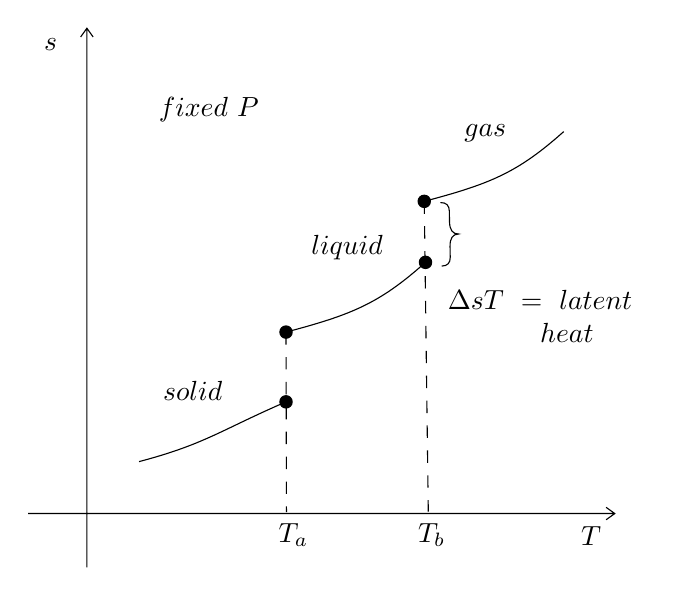
\begin{tikzpicture}[x=0.75pt,y=0.75pt,yscale=-0.6,xscale=0.6]
%uncomment if require: \path (0,433); %set diagram left start at 0, and has height of 433

%Shape: Axis 2D [id:dp34042133393206886]
\draw  (72,390.7) -- (543,390.7)(119.1,1) -- (119.1,434) (536,385.7) -- (543,390.7) -- (536,395.7) (114.1,8) -- (119.1,1) -- (124.1,8)  ;
%Straight Lines [id:da1379576233427211]
\draw  [dash pattern={on 4.5pt off 4.5pt}]  (390,140) -- (393.24,389.13) ;


%Straight Lines [id:da6702336744569144]
\draw  [dash pattern={on 4.5pt off 4.5pt}]  (279,245) -- (279.35,389.47) ;


%Curve Lines [id:da832017125366147]
\draw    (161,349) .. controls (214,335) and (226,324) .. (279,301) ;


%Curve Lines [id:da5776051073571846]
\draw    (279,245) .. controls (332,231) and (354,222) .. (391,189) ;


%Curve Lines [id:da7340600546503095]
\draw    (390,140) .. controls (443,126) and (465,117) .. (502,84) ;


%Shape: Circle [id:dp11951484801542822]
\draw  [color={rgb, 255:red, 0; green, 0; blue, 0 }  ,draw opacity=1 ][fill={rgb, 255:red, 0; green, 0; blue, 0 }  ,fill opacity=1 ] (274.05,245) .. controls (274.05,242.26) and (276.26,240.05) .. (279,240.05) .. controls (281.74,240.05) and (283.95,242.26) .. (283.95,245) .. controls (283.95,247.74) and (281.74,249.95) .. (279,249.95) .. controls (276.26,249.95) and (274.05,247.74) .. (274.05,245) -- cycle ;
%Shape: Circle [id:dp6821519031317774]
\draw  [color={rgb, 255:red, 0; green, 0; blue, 0 }  ,draw opacity=1 ][fill={rgb, 255:red, 0; green, 0; blue, 0 }  ,fill opacity=1 ] (274.05,301) .. controls (274.05,298.26) and (276.26,296.05) .. (279,296.05) .. controls (281.74,296.05) and (283.95,298.26) .. (283.95,301) .. controls (283.95,303.74) and (281.74,305.95) .. (279,305.95) .. controls (276.26,305.95) and (274.05,303.74) .. (274.05,301) -- cycle ;
%Shape: Circle [id:dp47646574064875924]
\draw  [color={rgb, 255:red, 0; green, 0; blue, 0 }  ,draw opacity=1 ][fill={rgb, 255:red, 0; green, 0; blue, 0 }  ,fill opacity=1 ] (386.05,189) .. controls (386.05,186.26) and (388.26,184.05) .. (391,184.05) .. controls (393.74,184.05) and (395.95,186.26) .. (395.95,189) .. controls (395.95,191.74) and (393.74,193.95) .. (391,193.95) .. controls (388.26,193.95) and (386.05,191.74) .. (386.05,189) -- cycle ;
%Shape: Circle [id:dp6226666771141686]
\draw  [color={rgb, 255:red, 0; green, 0; blue, 0 }  ,draw opacity=1 ][fill={rgb, 255:red, 0; green, 0; blue, 0 }  ,fill opacity=1 ] (385.05,140) .. controls (385.05,137.26) and (387.26,135.05) .. (390,135.05) .. controls (392.74,135.05) and (394.95,137.26) .. (394.95,140) .. controls (394.95,142.74) and (392.74,144.95) .. (390,144.95) .. controls (387.26,144.95) and (385.05,142.74) .. (385.05,140) -- cycle ;
%Shape: Brace [id:dp5923029079093556]
\draw   (404,192) .. controls (408.67,191.91) and (410.95,189.53) .. (410.86,184.86) -- (410.7,176.36) .. controls (410.57,169.69) and (412.83,166.32) .. (417.5,166.23) .. controls (412.83,166.32) and (410.43,163.03) .. (410.3,156.37)(410.36,159.36) -- (410.14,147.86) .. controls (410.05,143.19) and (407.67,140.91) .. (403,141) ;

% Text Node
\draw (204,292) node   {$solid$};
% Text Node
\draw (328,177) node   {$liquid$};
% Text Node
\draw (439,85) node   {$gas$};
% Text Node
\draw (90,14) node   {$s$};
% Text Node
\draw (524,409) node   {$T$};
% Text Node
\draw (285,408) node   {$T_{a}$};
% Text Node
\draw (396,408) node   {$T_{b}$};
% Text Node
\draw (483,235) node   {$ \begin{array}{l}
\Delta sT\ =\ latent\\
\quad \quad \quad \ heat\ \quad
\end{array}$};
% Text Node
\draw (217,66) node   {$fixed\ P$};


\end{tikzpicture}

\caption{\label{fig:2_4} Description.}
\end{figure}

We can also fix the temperature \emph{T} and look at the variation of \emph{P} (Figure \ref{fig:2_5}) and we have (Figure \ref{fig:2_6}) \( v= \qty(\pdv{g}{P} )_T > 0  \) :
\begin{equation}
  \qty(\pdv[2]{g}{P} ) = \qty(\pdv{U}{P} )_T = -v k_T < 0
  \label{eq:}
\end{equation}

\begin{figure}[h!]
\centering


\tikzset{every picture/.style={line width=0.75pt}} %set default line width to 0.75pt

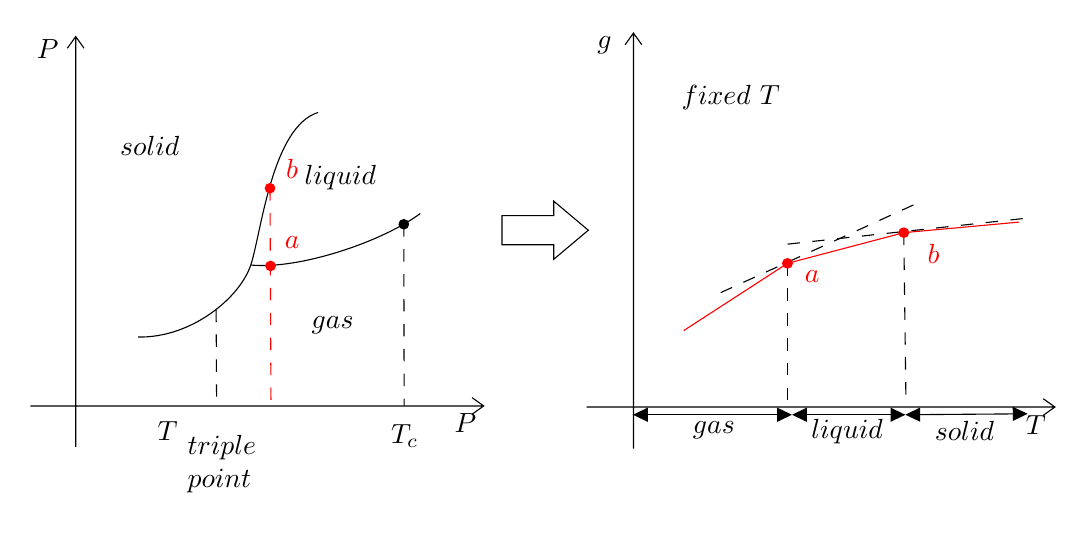
\begin{tikzpicture}[x=0.75pt,y=0.75pt,yscale=-0.8,xscale=0.8]
%uncomment if require: \path (0,433); %set diagram left start at 0, and has height of 433

%Shape: Axis 2D [id:dp1498177147678551]
\draw  (8,259.33) -- (281,259.33)(35.3,36.89) -- (35.3,284.04) (274,254.33) -- (281,259.33) -- (274,264.33) (30.3,43.89) -- (35.3,36.89) -- (40.3,43.89)  ;
%Curve Lines [id:da38606379255675294]
\draw    (72.92,217.83) .. controls (105.38,218.4) and (134.36,193.86) .. (140.73,174.45) .. controls (147.11,155.05) and (153.48,91.12) .. (181.31,82.56) ;


%Curve Lines [id:da5094178700447584]
\draw    (140.73,174.45) .. controls (169.71,177.31) and (219.59,160.6) .. (242.78,143.47) ;


%Straight Lines [id:da9253633278224371]
\draw  [dash pattern={on 4.5pt off 4.5pt}]  (119.87,201.28) -- (120.16,259.46) ;


%Straight Lines [id:da34937077008661355]
\draw  [dash pattern={on 4.5pt off 4.5pt}]  (232.89,149.91) -- (233.09,259.2) ;


%Straight Lines [id:da8284127524587958]
\draw [color={rgb, 255:red, 255; green, 0; blue, 0 }  ,draw opacity=1 ] [dash pattern={on 4.5pt off 4.5pt}]  (152.32,128.22) -- (152.9,259.5) ;


%Shape: Ellipse [id:dp661470809857147]
\draw  [color={rgb, 255:red, 255; green, 0; blue, 0 }  ,draw opacity=1 ][fill={rgb, 255:red, 255; green, 0; blue, 0 }  ,fill opacity=1 ] (149.45,128.22) .. controls (149.45,126.66) and (150.74,125.39) .. (152.32,125.39) .. controls (153.91,125.39) and (155.2,126.66) .. (155.2,128.22) .. controls (155.2,129.78) and (153.91,131.05) .. (152.32,131.05) .. controls (150.74,131.05) and (149.45,129.78) .. (149.45,128.22) -- cycle ;
%Shape: Ellipse [id:dp15843839054523723]
\draw  [color={rgb, 255:red, 255; green, 0; blue, 0 }  ,draw opacity=1 ][fill={rgb, 255:red, 255; green, 0; blue, 0 }  ,fill opacity=1 ] (149.77,175.01) .. controls (149.77,173.45) and (151.06,172.18) .. (152.65,172.18) .. controls (154.23,172.18) and (155.52,173.45) .. (155.52,175.01) .. controls (155.52,176.57) and (154.23,177.84) .. (152.65,177.84) .. controls (151.06,177.84) and (149.77,176.57) .. (149.77,175.01) -- cycle ;
%Shape: Ellipse [id:dp32169374942348206]
\draw  [color={rgb, 255:red, 0; green, 0; blue, 0 }  ,draw opacity=1 ][fill={rgb, 255:red, 0; green, 0; blue, 0 }  ,fill opacity=1 ] (230.02,149.91) .. controls (230.02,148.35) and (231.31,147.08) .. (232.89,147.08) .. controls (234.48,147.08) and (235.76,148.35) .. (235.76,149.91) .. controls (235.76,151.47) and (234.48,152.74) .. (232.89,152.74) .. controls (231.31,152.74) and (230.02,151.47) .. (230.02,149.91) -- cycle ;
%Shape: Axis 2D [id:dp07025604911421235]
\draw  (343,259.98) -- (625,259.98)(371.2,34.77) -- (371.2,285) (618,254.98) -- (625,259.98) -- (618,264.98) (366.2,41.77) -- (371.2,34.77) -- (376.2,41.77)  ;
%Straight Lines [id:da8800071085611229]
\draw  [dash pattern={on 4.5pt off 4.5pt}]  (533.99,154.97) -- (535.34,259.07) ;


%Straight Lines [id:da34380509061608333]
\draw  [dash pattern={on 4.5pt off 4.5pt}]  (463.94,173.46) -- (463.94,260.15) ;


%Straight Lines [id:da1088483295937368]
\draw [color={rgb, 255:red, 255; green, 0; blue, 0 }  ,draw opacity=1 ]   (401.45,213.96) -- (463.94,173.46) -- (533.99,154.97) -- (603.45,148.61) ;


%Straight Lines [id:da8846445499976445]
\draw  [dash pattern={on 4.5pt off 4.5pt}]  (423.75,191.08) -- (540.02,138.19) ;


%Straight Lines [id:da2618488487813475]
\draw    (372.88,264.63) -- (464.67,264.63) ;
\draw [shift={(466.67,264.63)}, rotate = 180] [fill={rgb, 255:red, 0; green, 0; blue, 0 }  ][line width=0.75]  [draw opacity=0] (8.93,-4.29) -- (0,0) -- (8.93,4.29) -- cycle    ;
\draw [shift={(370.88,264.63)}, rotate = 0] [fill={rgb, 255:red, 0; green, 0; blue, 0 }  ][line width=0.75]  [draw opacity=0] (8.93,-4.29) -- (0,0) -- (8.93,4.29) -- cycle    ;
%Straight Lines [id:da011061969013948403]
\draw    (468.67,264.63) -- (532.93,264.63) ;
\draw [shift={(534.93,264.63)}, rotate = 180] [fill={rgb, 255:red, 0; green, 0; blue, 0 }  ][line width=0.75]  [draw opacity=0] (8.93,-4.29) -- (0,0) -- (8.93,4.29) -- cycle    ;
\draw [shift={(466.67,264.63)}, rotate = 0] [fill={rgb, 255:red, 0; green, 0; blue, 0 }  ][line width=0.75]  [draw opacity=0] (8.93,-4.29) -- (0,0) -- (8.93,4.29) -- cycle    ;
%Straight Lines [id:da8783042264268455]
\draw    (536.93,264.61) -- (606.57,264.07) ;
\draw [shift={(608.57,264.05)}, rotate = 539.55] [fill={rgb, 255:red, 0; green, 0; blue, 0 }  ][line width=0.75]  [draw opacity=0] (8.93,-4.29) -- (0,0) -- (8.93,4.29) -- cycle    ;
\draw [shift={(534.93,264.63)}, rotate = 359.55] [fill={rgb, 255:red, 0; green, 0; blue, 0 }  ][line width=0.75]  [draw opacity=0] (8.93,-4.29) -- (0,0) -- (8.93,4.29) -- cycle    ;
%Straight Lines [id:da3414026804600607]
\draw  [dash pattern={on 4.5pt off 4.5pt}]  (463.98,161.88) -- (607.67,146.28) ;


%Shape: Ellipse [id:dp5732735899807143]
\draw  [color={rgb, 255:red, 255; green, 0; blue, 0 }  ,draw opacity=1 ][fill={rgb, 255:red, 255; green, 0; blue, 0 }  ,fill opacity=1 ] (531.03,154.97) .. controls (531.03,153.39) and (532.36,152.11) .. (533.99,152.11) .. controls (535.63,152.11) and (536.96,153.39) .. (536.96,154.97) .. controls (536.96,156.55) and (535.63,157.83) .. (533.99,157.83) .. controls (532.36,157.83) and (531.03,156.55) .. (531.03,154.97) -- cycle ;
%Shape: Ellipse [id:dp995516034298798]
\draw  [color={rgb, 255:red, 255; green, 0; blue, 0 }  ,draw opacity=1 ][fill={rgb, 255:red, 255; green, 0; blue, 0 }  ,fill opacity=1 ] (460.98,173.46) .. controls (460.98,171.88) and (462.3,170.6) .. (463.94,170.6) .. controls (465.58,170.6) and (466.91,171.88) .. (466.91,173.46) .. controls (466.91,175.05) and (465.58,176.33) .. (463.94,176.33) .. controls (462.3,176.33) and (460.98,175.05) .. (460.98,173.46) -- cycle ;
%Right Arrow [id:dp3505935332690939]
\draw  [color={rgb, 255:red, 0; green, 0; blue, 0 }  ,draw opacity=1 ][fill={rgb, 255:red, 255; green, 255; blue, 255 }  ,fill opacity=1 ] (292,144.75) -- (323.2,144.75) -- (323.2,136) -- (344,153.5) -- (323.2,171) -- (323.2,162.25) -- (292,162.25) -- cycle ;

% Text Node
\draw (79.87,102.53) node   {$solid$};
% Text Node
\draw (194.64,121.94) node   {$liquid$};
% Text Node
\draw (190,210.98) node   {$gas$};
% Text Node
\draw (165.66,160.75) node [color={rgb, 255:red, 255; green, 0; blue, 0 }  ,opacity=1 ]  {$a$};
% Text Node
\draw (165.66,116.8) node [color={rgb, 255:red, 255; green, 0; blue, 0 }  ,opacity=1 ]  {$b$};
% Text Node
\draw (121.61,291.58) node   {$T_{ \begin{array}{l}
triple\ \\
point
\end{array}}$};
% Text Node
\draw (233.47,277.58) node   {$T_{c}$};
% Text Node
\draw (18.43,44.31) node   {$P$};
% Text Node
\draw (269.99,269.77) node   {$P$};
% Text Node
\draw (570.52,274.6) node   {$solid$};
% Text Node
\draw (499.87,274.6) node   {$liquid$};
% Text Node
\draw (419.64,274.02) node   {$gas$};
% Text Node
\draw (478.91,181.56) node [color={rgb, 255:red, 255; green, 0; blue, 0 }  ,opacity=1 ]  {$a$};
% Text Node
\draw (551.96,167.69) node [color={rgb, 255:red, 255; green, 0; blue, 0 }  ,opacity=1 ]  {$b$};
% Text Node
\draw (353.78,42.28) node   {$g$};
% Text Node
\draw (613.62,270.55) node   {$T$};
% Text Node
\draw (429.82,73.49) node   {$fixed\ T$};


\end{tikzpicture}

\caption{\label{fig:2_5} Description.}
\end{figure}

\begin{figure}[h!]
\centering


\tikzset{every picture/.style={line width=0.75pt}} %set default line width to 0.75pt

\begin{tikzpicture}[x=0.75pt,y=0.75pt,yscale=-0.6,xscale=0.6]
%uncomment if require: \path (0,433); %set diagram left start at 0, and has height of 433

%Shape: Axis 2D [id:dp34042133393206886]
\draw  (72,390.7) -- (543,390.7)(119.1,1) -- (119.1,434) (536,385.7) -- (543,390.7) -- (536,395.7) (114.1,8) -- (119.1,1) -- (124.1,8)  ;
%Straight Lines [id:da1379576233427211]
\draw  [dash pattern={on 4.5pt off 4.5pt}]  (391.62,264.57) -- (393.24,389.13) ;


%Straight Lines [id:da6702336744569144]
\draw  [dash pattern={on 4.5pt off 4.5pt}]  (278,134) -- (279.35,389.47) ;


%Curve Lines [id:da832017125366147]
\draw    (154,54) .. controls (175,84) and (220,123) .. (278,134) ;


%Curve Lines [id:da5776051073571846]
\draw    (278.62,202.57) .. controls (298.62,233.57) and (343.62,266.57) .. (391.62,264.57) ;


%Curve Lines [id:da7340600546503095]
\draw    (394,315) .. controls (426,341) and (456,371) .. (509,367) ;


%Shape: Circle [id:dp11951484801542822]
\draw  [color={rgb, 255:red, 0; green, 0; blue, 0 }  ,draw opacity=1 ][fill={rgb, 255:red, 0; green, 0; blue, 0 }  ,fill opacity=1 ] (273.67,202.57) .. controls (273.67,199.83) and (275.89,197.61) .. (278.62,197.61) .. controls (281.36,197.61) and (283.58,199.83) .. (283.58,202.57) .. controls (283.58,205.3) and (281.36,207.52) .. (278.62,207.52) .. controls (275.89,207.52) and (273.67,205.3) .. (273.67,202.57) -- cycle ;
%Shape: Circle [id:dp6821519031317774]
\draw  [color={rgb, 255:red, 0; green, 0; blue, 0 }  ,draw opacity=1 ][fill={rgb, 255:red, 0; green, 0; blue, 0 }  ,fill opacity=1 ] (273.05,134) .. controls (273.05,131.26) and (275.26,129.05) .. (278,129.05) .. controls (280.74,129.05) and (282.95,131.26) .. (282.95,134) .. controls (282.95,136.74) and (280.74,138.95) .. (278,138.95) .. controls (275.26,138.95) and (273.05,136.74) .. (273.05,134) -- cycle ;
%Shape: Circle [id:dp47646574064875924]
\draw  [color={rgb, 255:red, 0; green, 0; blue, 0 }  ,draw opacity=1 ][fill={rgb, 255:red, 0; green, 0; blue, 0 }  ,fill opacity=1 ] (386.67,264.57) .. controls (386.67,261.83) and (388.89,259.61) .. (391.62,259.61) .. controls (394.36,259.61) and (396.58,261.83) .. (396.58,264.57) .. controls (396.58,267.3) and (394.36,269.52) .. (391.62,269.52) .. controls (388.89,269.52) and (386.67,267.3) .. (386.67,264.57) -- cycle ;
%Shape: Circle [id:dp6226666771141686]
\draw  [color={rgb, 255:red, 0; green, 0; blue, 0 }  ,draw opacity=1 ][fill={rgb, 255:red, 0; green, 0; blue, 0 }  ,fill opacity=1 ] (389.05,315) .. controls (389.05,312.26) and (391.26,310.05) .. (394,310.05) .. controls (396.74,310.05) and (398.95,312.26) .. (398.95,315) .. controls (398.95,317.74) and (396.74,319.95) .. (394,319.95) .. controls (391.26,319.95) and (389.05,317.74) .. (389.05,315) -- cycle ;

% Text Node
\draw (454,410) node   {$solid$};
% Text Node
\draw (337,411) node   {$liquid$};
% Text Node
\draw (194,410) node   {$gas$};
% Text Node
\draw (90,14) node   {$v$};
% Text Node
\draw (524,409) node   {$P$};
% Text Node
\draw (217,66) node   {$fixed\ P$};
% Text Node
\draw (243.97,213.87) node [color={rgb, 255:red, 255; green, 0; blue, 0 }  ,opacity=1 ]  {$a$};
% Text Node
\draw (423.97,248.87) node [color={rgb, 255:red, 255; green, 0; blue, 0 }  ,opacity=1 ]  {$b$};


\end{tikzpicture}

\caption{\label{fig:2_6} Description.}
\end{figure}

\section{Second order phase transition}
There are other cases in which we do not have these effects, as in Figure \ref{fig:2_7}. This is different from the previous situation in which we had a jump:
\begin{subequations}
\begin{align}
  \qty(\pdv{g}{T} )_P &= -s \\
  \qty(\pdv{g}{P} )_T &= v
\end{align}
\label{}
\end{subequations}
This implies:
\begin{equation}
  \qty(\pdv{g}{T}{P}  ) = \qty(\pdv{v}{T} )_P = v_{\alpha p}
  \label{eq:}
\end{equation}
An example is \emph{superconductivity}.


\begin{figure}[h!]
\begin{minipage}[c]{0.5\linewidth}
\centering
\subfloat[][Description]{


\tikzset{every picture/.style={line width=0.75pt}} %set default line width to 0.75pt

\begin{tikzpicture}[x=0.75pt,y=0.75pt,yscale=-0.4,xscale=0.4]
%uncomment if require: \path (0,433); %set diagram left start at 0, and has height of 433

%Shape: Axis 2D [id:dp34042133393206886]
\draw  (72,390.7) -- (543,390.7)(119.1,1) -- (119.1,434) (536,385.7) -- (543,390.7) -- (536,395.7) (114.1,8) -- (119.1,1) -- (124.1,8)  ;
%Straight Lines [id:da6702336744569144]
\draw  [dash pattern={on 4.5pt off 4.5pt}]  (301,106) -- (303,391) ;


%Curve Lines [id:da832017125366147]
\draw    (178,78) .. controls (309,90) and (446,145) .. (470,309) ;


%Shape: Circle [id:dp6821519031317774]
\draw  [color={rgb, 255:red, 0; green, 0; blue, 0 }  ,draw opacity=1 ][fill={rgb, 255:red, 0; green, 0; blue, 0 }  ,fill opacity=1 ] (296.05,106) .. controls (296.05,103.26) and (298.26,101.05) .. (301,101.05) .. controls (303.74,101.05) and (305.95,103.26) .. (305.95,106) .. controls (305.95,108.74) and (303.74,110.95) .. (301,110.95) .. controls (298.26,110.95) and (296.05,108.74) .. (296.05,106) -- cycle ;

% Text Node
\draw (93,24) node   {$g$};
% Text Node
\draw (524,409) node   {$T$};
% Text Node
\draw (308,419) node   {$T_{a}$};


\end{tikzpicture}

    \label{fig:} }
\end{minipage}
\begin{minipage}[]{0.5\linewidth}
\centering
\subfloat[][Description]{


\tikzset{every picture/.style={line width=0.75pt}} %set default line width to 0.75pt

\begin{tikzpicture}[x=0.75pt,y=0.75pt,yscale=-0.4,xscale=0.4]
%uncomment if require: \path (0,433); %set diagram left start at 0, and has height of 433

%Shape: Axis 2D [id:dp34042133393206886]
\draw  (72,390.7) -- (543,390.7)(119.1,1) -- (119.1,434) (536,385.7) -- (543,390.7) -- (536,395.7) (114.1,8) -- (119.1,1) -- (124.1,8)  ;
%Straight Lines [id:da6702336744569144]
\draw  [dash pattern={on 4.5pt off 4.5pt}]  (301,169) -- (303,391) ;


%Curve Lines [id:da832017125366147]
\draw    (152,330) .. controls (234,314) and (270,266) .. (301,169) ;


%Shape: Circle [id:dp6821519031317774]
\draw  [color={rgb, 255:red, 0; green, 0; blue, 0 }  ,draw opacity=1 ][fill={rgb, 255:red, 0; green, 0; blue, 0 }  ,fill opacity=1 ] (296.05,169) .. controls (296.05,166.26) and (298.26,164.05) .. (301,164.05) .. controls (303.74,164.05) and (305.95,166.26) .. (305.95,169) .. controls (305.95,171.74) and (303.74,173.95) .. (301,173.95) .. controls (298.26,173.95) and (296.05,171.74) .. (296.05,169) -- cycle ;
%Straight Lines [id:da1662494918814228]
\draw    (301,169) -- (451,88) ;



% Text Node
\draw (93,24) node   {$s$};
% Text Node
\draw (524,409) node   {$T$};
% Text Node
\draw (308,419) node   {$T_{a}$};


\end{tikzpicture}

    \label{fig:} }
\end{minipage}
\\
\begin{minipage}[c]{0.5\linewidth}
\centering
\subfloat[][Description]{


\tikzset{every picture/.style={line width=0.75pt}} %set default line width to 0.75pt

\begin{tikzpicture}[x=0.75pt,y=0.75pt,yscale=-0.4,xscale=0.4]
%uncomment if require: \path (0,433); %set diagram left start at 0, and has height of 433

%Shape: Axis 2D [id:dp34042133393206886]
\draw  (72,390.7) -- (543,390.7)(119.1,1) -- (119.1,434) (536,385.7) -- (543,390.7) -- (536,395.7) (114.1,8) -- (119.1,1) -- (124.1,8)  ;
%Straight Lines [id:da6702336744569144]
\draw  [dash pattern={on 4.5pt off 4.5pt}]  (301,169) -- (303,391) ;


%Shape: Circle [id:dp6821519031317774]
\draw  [color={rgb, 255:red, 0; green, 0; blue, 0 }  ,draw opacity=1 ][fill={rgb, 255:red, 0; green, 0; blue, 0 }  ,fill opacity=1 ] (296.05,169) .. controls (296.05,166.26) and (298.26,164.05) .. (301,164.05) .. controls (303.74,164.05) and (305.95,166.26) .. (305.95,169) .. controls (305.95,171.74) and (303.74,173.95) .. (301,173.95) .. controls (298.26,173.95) and (296.05,171.74) .. (296.05,169) -- cycle ;
%Straight Lines [id:da1662494918814228]
\draw    (301,169) -- (451,88) ;


%Straight Lines [id:da8938048927675745]
\draw    (301,169) -- (191,331) ;



% Text Node
\draw (93,24) node   {$v$};
% Text Node
\draw (524,409) node   {$P$};
% Text Node
\draw (308,419) node   {$T_{a}$};


\end{tikzpicture}

    \label{fig:} }
\end{minipage}
\begin{minipage}[]{0.5\linewidth}
\centering
\subfloat[][Description]{


\tikzset{every picture/.style={line width=0.75pt}} %set default line width to 0.75pt

\begin{tikzpicture}[x=0.75pt,y=0.75pt,yscale=-0.4,xscale=0.4]
%uncomment if require: \path (0,433); %set diagram left start at 0, and has height of 433

%Shape: Axis 2D [id:dp34042133393206886]
\draw  (72,390.7) -- (543,390.7)(119.1,1) -- (119.1,434) (536,385.7) -- (543,390.7) -- (536,395.7) (114.1,8) -- (119.1,1) -- (124.1,8)  ;
%Straight Lines [id:da6702336744569144]
\draw  [dash pattern={on 4.5pt off 4.5pt}]  (300,102) -- (303,391) ;


%Shape: Circle [id:dp6821519031317774]
\draw  [color={rgb, 255:red, 0; green, 0; blue, 0 }  ,draw opacity=1 ][fill={rgb, 255:red, 0; green, 0; blue, 0 }  ,fill opacity=1 ] (295.05,106.95) .. controls (295.05,104.22) and (297.26,102) .. (300,102) .. controls (302.74,102) and (304.95,104.22) .. (304.95,106.95) .. controls (304.95,109.69) and (302.74,111.91) .. (300,111.91) .. controls (297.26,111.91) and (295.05,109.69) .. (295.05,106.95) -- cycle ;
%Straight Lines [id:da1662494918814228]
\draw    (303,293) -- (453,212) ;


%Curve Lines [id:da3323852489584005]
\draw    (153,262) .. controls (198,248) and (293,190) .. (300,102) ;



% Text Node
\draw (93,24) node   {$c_{P}$};
% Text Node
\draw (524,409) node   {$T$};
% Text Node
\draw (308,419) node   {$T_{a}$};


\end{tikzpicture}

    \label{fig:2_7_4} }
\end{minipage}
\caption{\label{fig:2_7} Description}
\end{figure}

If we look for example at the specific heat in Figure \ref{fig:2_7_4}, it represent the transition from superconduction.

The critical point is special beacause there is not a jump, so we can go continuously from gas to liquid. The response function when we plot this point shows that the specific heat diverges.
The transitions are classified in the first order transition and continuous transition. The superfluid transition is a transition where the second derivative of the thermodynamic potential diverges. There are many phase transitions that can be classified in different ways.
We note that at the coexistence line we increase V, but the pression remains constant. At the coexistence line we see bubbles. It is the density that is changing locally, the bubbles becames bigger and bigger and at the \( V_G \) , becames a liquid.


\section{Helmholtz free-energy}
Consider \( A = A (T,V,N) \), here \emph{P} is replaced by \emph{V} which is discontinuous at the first order transition. Moreover \( P > 0 \)  implies \( \partial{A}/\partial{V} < 0   \) and
\begin{equation}
  k_T = -\frac{1}{V} \qty(\pdv{V}{P} )_T = -\frac{1}{V} \qty(\pdv{P}{V} )_T = \frac{1}{V} \qty(\pdv[2]{A}{V} )_T > 0
  \label{eq:}
\end{equation}
\emph{A} is an overall convex function of \emph{V}.
The behaviour of \emph{A} when there is a first order phase transition is as in Figure \ref{fig:2_8_1}. The linear sector becomes an horizontal one in the \( P = - (\partial{A}/\partial{V}  )_T = P (V) \) curve (Figure \ref{fig:2_8_2}).




\begin{figure}[h!]
\begin{minipage}[c]{0.5\linewidth}
\centering
\subfloat[][Description]{


\tikzset{every picture/.style={line width=0.75pt}} %set default line width to 0.75pt

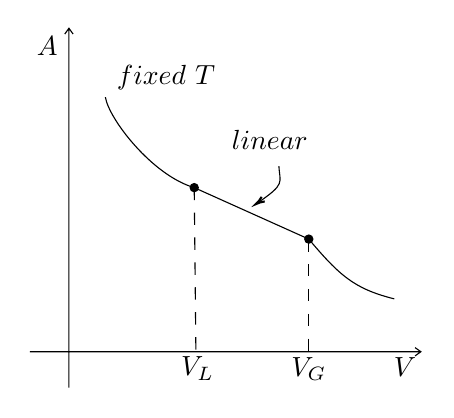
\begin{tikzpicture}[x=0.75pt,y=0.75pt,yscale=-0.4,xscale=0.4]
%uncomment if require: \path (0,433); %set diagram left start at 0, and has height of 433

%Shape: Axis 2D [id:dp34042133393206886]
\draw  (72,390.7) -- (543,390.7)(119.1,1) -- (119.1,434) (536,385.7) -- (543,390.7) -- (536,395.7) (114.1,8) -- (119.1,1) -- (124.1,8)  ;
%Straight Lines [id:da6702336744569144]
\draw  [dash pattern={on 4.5pt off 4.5pt}]  (270,193) -- (272,390) ;


%Shape: Circle [id:dp6821519031317774]
\draw  [color={rgb, 255:red, 0; green, 0; blue, 0 }  ,draw opacity=1 ][fill={rgb, 255:red, 0; green, 0; blue, 0 }  ,fill opacity=1 ] (265.05,193) .. controls (265.05,190.26) and (267.26,188.05) .. (270,188.05) .. controls (272.74,188.05) and (274.95,190.26) .. (274.95,193) .. controls (274.95,195.74) and (272.74,197.95) .. (270,197.95) .. controls (267.26,197.95) and (265.05,195.74) .. (265.05,193) -- cycle ;
%Straight Lines [id:da1662494918814228]
\draw    (270,193) -- (408,255) ;


%Straight Lines [id:da7053989083670136]
\draw  [dash pattern={on 4.5pt off 4.5pt}]  (408,255) -- (408,391) ;


%Curve Lines [id:da6886563534922254]
\draw    (408,255) .. controls (445,299) and (463,315) .. (511,327) ;


%Curve Lines [id:da48601947297403236]
\draw    (163,84) .. controls (167,110) and (219,178) .. (270,193) ;


%Shape: Circle [id:dp988494671197904]
\draw  [color={rgb, 255:red, 0; green, 0; blue, 0 }  ,draw opacity=1 ][fill={rgb, 255:red, 0; green, 0; blue, 0 }  ,fill opacity=1 ] (403.05,255) .. controls (403.05,252.26) and (405.26,250.05) .. (408,250.05) .. controls (410.74,250.05) and (412.95,252.26) .. (412.95,255) .. controls (412.95,257.74) and (410.74,259.95) .. (408,259.95) .. controls (405.26,259.95) and (403.05,257.74) .. (403.05,255) -- cycle ;
%Curve Lines [id:da30431708024345916]
\draw    (372,167) .. controls (372.99,187.69) and (380.76,188) .. (345.63,211.89) ;
\draw [shift={(344,213)}, rotate = 325.95] [color={rgb, 255:red, 0; green, 0; blue, 0 }  ][line width=0.75]    (10.93,-3.29) .. controls (6.95,-1.4) and (3.31,-0.3) .. (0,0) .. controls (3.31,0.3) and (6.95,1.4) .. (10.93,3.29)   ;


% Text Node
\draw (93,23) node   {$A$};
% Text Node
\draw (524,409) node   {$V$};
% Text Node
\draw (274,411) node   {$V_{L}$};
% Text Node
\draw (408,412) node   {$V_{G}$};
% Text Node
\draw (361,135) node   {$linear$};
% Text Node
\draw (236,60) node   {$fixed\ T$};


\end{tikzpicture}

    \label{fig:2_8_1} }
\end{minipage}
\begin{minipage}[]{0.5\linewidth}
\centering
\subfloat[][Description]{


\tikzset{every picture/.style={line width=0.75pt}} %set default line width to 0.75pt

\begin{tikzpicture}[x=0.75pt,y=0.75pt,yscale=-0.4,xscale=0.4]
%uncomment if require: \path (0,433); %set diagram left start at 0, and has height of 433

%Shape: Axis 2D [id:dp34042133393206886]
\draw  (72,390.7) -- (543,390.7)(119.1,1) -- (119.1,434) (536,385.7) -- (543,390.7) -- (536,395.7) (114.1,8) -- (119.1,1) -- (124.1,8)  ;
%Straight Lines [id:da6702336744569144]
\draw  [dash pattern={on 4.5pt off 4.5pt}]  (272,254) -- (272,390) ;


%Shape: Circle [id:dp6821519031317774]
\draw  [color={rgb, 255:red, 0; green, 0; blue, 0 }  ,draw opacity=1 ][fill={rgb, 255:red, 0; green, 0; blue, 0 }  ,fill opacity=1 ] (267.05,254) .. controls (267.05,251.26) and (269.26,249.05) .. (272,249.05) .. controls (274.74,249.05) and (276.95,251.26) .. (276.95,254) .. controls (276.95,256.74) and (274.74,258.95) .. (272,258.95) .. controls (269.26,258.95) and (267.05,256.74) .. (267.05,254) -- cycle ;
%Straight Lines [id:da1662494918814228]
\draw    (272,254) -- (408,255) ;


%Straight Lines [id:da7053989083670136]
\draw  [dash pattern={on 4.5pt off 4.5pt}]  (408,255) -- (408,391) ;


%Curve Lines [id:da6886563534922254]
\draw    (408,255) .. controls (445,299) and (463,315) .. (511,327) ;


%Curve Lines [id:da48601947297403236]
\draw    (165,145) .. controls (169,171) and (221,239) .. (272,254) ;


%Shape: Circle [id:dp988494671197904]
\draw  [color={rgb, 255:red, 0; green, 0; blue, 0 }  ,draw opacity=1 ][fill={rgb, 255:red, 0; green, 0; blue, 0 }  ,fill opacity=1 ] (403.05,255) .. controls (403.05,252.26) and (405.26,250.05) .. (408,250.05) .. controls (410.74,250.05) and (412.95,252.26) .. (412.95,255) .. controls (412.95,257.74) and (410.74,259.95) .. (408,259.95) .. controls (405.26,259.95) and (403.05,257.74) .. (403.05,255) -- cycle ;

% Text Node
\draw (93,23) node   {$P$};
% Text Node
\draw (524,409) node   {$V$};
% Text Node
\draw (274,411) node   {$V_{L}$};
% Text Node
\draw (408,412) node   {$V_{G}$};


\end{tikzpicture}

    \label{fig:2_8_2} }
\end{minipage}
\caption{\label{fig:2_8} Description}
\end{figure}



\section{Critical points}
At the critical point \( (P_c,T_c) \) the system can pass from the liquid to the gas phase (and viceversa) in a continuous way
\begin{equation}
  \Delta s = \Delta v = 0
  \label{eq:}
\end{equation}
Usually critical points are end point of first order transition phases. Why there is no critical point between solid and liquid? The crossover between phases having the same symmetry define the Landau point. There is a break of symmetry, for instance we can think about the structure of the bravais lattice. Instead, from gas to liquid symmetries are not broken.

\begin{figure}[h!]
\centering


\tikzset{every picture/.style={line width=0.75pt}} %set default line width to 0.75pt

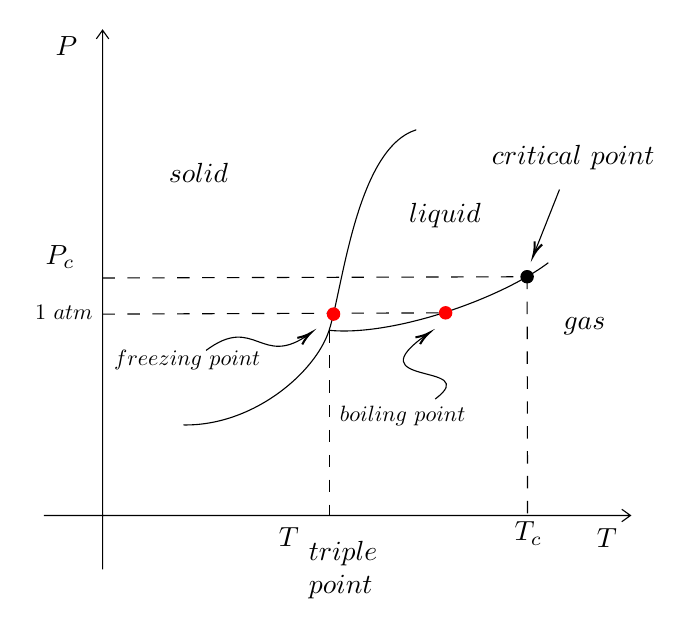
\begin{tikzpicture}[x=0.75pt,y=0.75pt,yscale=-0.6,xscale=0.6]
%uncomment if require: \path (0,433); %set diagram left start at 0, and has height of 433

%Shape: Axis 2D [id:dp34042133393206886]
\draw  (72,390.7) -- (543,390.7)(119.1,1) -- (119.1,434) (536,385.7) -- (543,390.7) -- (536,395.7) (114.1,8) -- (119.1,1) -- (124.1,8)  ;
%Curve Lines [id:da2649058921866929]
\draw    (184,318) .. controls (240,319) and (290,276) .. (301,242) .. controls (312,208) and (323,96) .. (371,81) ;


%Curve Lines [id:da19336772925785306]
\draw    (301,242) .. controls (351,247) and (437.06,217.73) .. (477.06,187.73) ;


%Straight Lines [id:da1379576233427211]
\draw  [dash pattern={on 4.5pt off 4.5pt}]  (301,242) -- (301,390) ;


%Straight Lines [id:da6702336744569144]
\draw  [dash pattern={on 4.5pt off 4.5pt}]  (460,199) -- (460.35,390.47) ;


%Shape: Circle [id:dp768993062031393]
\draw  [color={rgb, 255:red, 255; green, 0; blue, 0 }  ,draw opacity=1 ][fill={rgb, 255:red, 255; green, 0; blue, 0 }  ,fill opacity=1 ] (389.6,227.98) .. controls (389.6,225.24) and (391.82,223.03) .. (394.55,223.03) .. controls (397.29,223.03) and (399.51,225.24) .. (399.51,227.98) .. controls (399.51,230.72) and (397.29,232.93) .. (394.55,232.93) .. controls (391.82,232.93) and (389.6,230.72) .. (389.6,227.98) -- cycle ;
%Curve Lines [id:da897292552339868]
\draw    (202.21,258.16) .. controls (241.81,228.46) and (246.13,273.25) .. (285.02,245.04) ;
\draw [shift={(286.21,244.16)}, rotate = 503.13] [color={rgb, 255:red, 0; green, 0; blue, 0 }  ][line width=0.75]    (10.93,-3.29) .. controls (6.95,-1.4) and (3.31,-0.3) .. (0,0) .. controls (3.31,0.3) and (6.95,1.4) .. (10.93,3.29)   ;

%Curve Lines [id:da43687585409049334]
\draw    (386.21,297.16) .. controls (426.01,267.31) and (318.3,287.95) .. (380.27,244.82) ;
\draw [shift={(381.21,244.16)}, rotate = 505.49] [color={rgb, 255:red, 0; green, 0; blue, 0 }  ][line width=0.75]    (10.93,-3.29) .. controls (6.95,-1.4) and (3.31,-0.3) .. (0,0) .. controls (3.31,0.3) and (6.95,1.4) .. (10.93,3.29)   ;

%Shape: Circle [id:dp07400034471483774]
\draw  [color={rgb, 255:red, 0; green, 0; blue, 0 }  ,draw opacity=1 ][fill={rgb, 255:red, 0; green, 0; blue, 0 }  ,fill opacity=1 ] (455.05,199) .. controls (455.05,196.26) and (457.26,194.05) .. (460,194.05) .. controls (462.74,194.05) and (464.95,196.26) .. (464.95,199) .. controls (464.95,201.74) and (462.74,203.95) .. (460,203.95) .. controls (457.26,203.95) and (455.05,201.74) .. (455.05,199) -- cycle ;
%Straight Lines [id:da29969851398494274]
\draw  [dash pattern={on 4.5pt off 4.5pt}]  (119,200) -- (460,199) ;


%Straight Lines [id:da602287698180992]
\draw  [dash pattern={on 4.5pt off 4.5pt}]  (119,229) -- (394.55,227.98) ;


%Shape: Circle [id:dp4330038061237751]
\draw  [color={rgb, 255:red, 255; green, 0; blue, 0 }  ,draw opacity=1 ][fill={rgb, 255:red, 255; green, 0; blue, 0 }  ,fill opacity=1 ] (299.6,228.98) .. controls (299.6,226.24) and (301.82,224.03) .. (304.55,224.03) .. controls (307.29,224.03) and (309.51,226.24) .. (309.51,228.98) .. controls (309.51,231.72) and (307.29,233.93) .. (304.55,233.93) .. controls (301.82,233.93) and (299.6,231.72) .. (299.6,228.98) -- cycle ;
%Straight Lines [id:da2746826747815124]
\draw    (486,129) -- (465.74,180.14) ;
\draw [shift={(465,182)}, rotate = 291.61] [color={rgb, 255:red, 0; green, 0; blue, 0 }  ][line width=0.75]    (10.93,-3.29) .. controls (6.95,-1.4) and (3.31,-0.3) .. (0,0) .. controls (3.31,0.3) and (6.95,1.4) .. (10.93,3.29)   ;


% Text Node
\draw (196,116) node   {$solid$};
% Text Node
\draw (394,150) node   {$liquid$};
% Text Node
\draw (506,239) node   {$gas$};
% Text Node
\draw (187,266.16) node [scale=0.8] {$freezing\ point$};
% Text Node
\draw (360,311.16) node  [scale=0.8] {$boiling\ point$};
% Text Node
\draw (310,431.16) node   {$T_{ \begin{array}{l}
triple\ \\
point
\end{array}}$};
% Text Node
\draw (461,405.16) node   {$T_{c}$};
% Text Node
\draw (90,14) node   {$P$};
% Text Node
\draw (524,409) node   {$T$};
% Text Node
\draw (497,103) node   {$critical\ point$};
% Text Node
\draw (88,228) node  [scale=0.8] {$1\ atm$};
% Text Node
\draw (85,183) node   {$P_{c}$};


\end{tikzpicture}

\caption{\label{fig:2_9} Description.}
\end{figure}



\section{Ferromagnetic system}



\begin{figure}[h!]
\centering


\tikzset{every picture/.style={line width=0.75pt}} %set default line width to 0.75pt

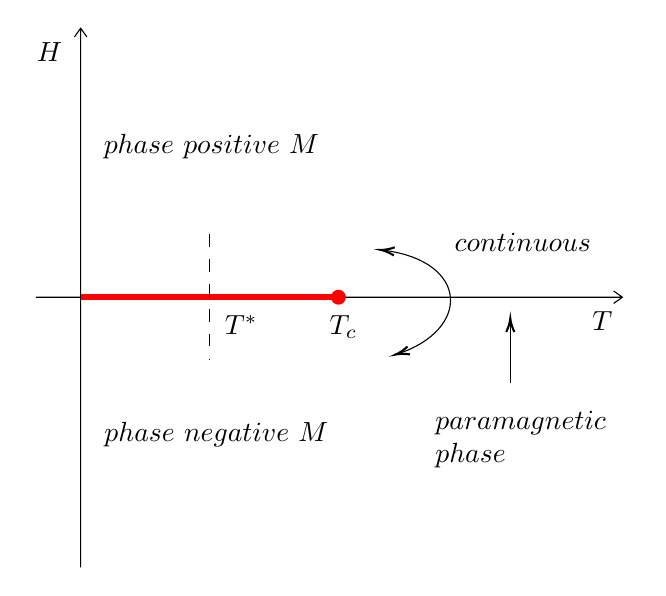
\begin{tikzpicture}[x=0.75pt,y=0.75pt,yscale=-0.6,xscale=0.6]
%uncomment if require: \path (0,433); %set diagram left start at 0, and has height of 433

%Shape: Axis 2D [id:dp34042133393206886]
\draw  (72,217) -- (543,217)(108,1) -- (108,434) (536,212) -- (543,217) -- (536,222) (103,8) -- (108,1) -- (113,8)  ;
%Straight Lines [id:da9551803962585098]
\draw [color={rgb, 255:red, 255; green, 0; blue, 0 }  ,draw opacity=1 ][line width=2.25]    (108,217) -- (315,217) ;


%Shape: Circle [id:dp40105900325823207]
\draw  [color={rgb, 255:red, 255; green, 0; blue, 0 }  ,draw opacity=1 ][fill={rgb, 255:red, 255; green, 0; blue, 0 }  ,fill opacity=1 ] (309.48,217) .. controls (309.48,213.95) and (311.95,211.48) .. (315,211.48) .. controls (318.05,211.48) and (320.52,213.95) .. (320.52,217) .. controls (320.52,220.05) and (318.05,222.52) .. (315,222.52) .. controls (311.95,222.52) and (309.48,220.05) .. (309.48,217) -- cycle ;
%Curve Lines [id:da3888044898644526]
\draw    (351.14,179.25) .. controls (420.32,188.05) and (421.38,243.07) .. (362.79,262.42) ;
\draw [shift={(361,263)}, rotate = 342.7] [color={rgb, 255:red, 0; green, 0; blue, 0 }  ][line width=0.75]    (10.93,-3.29) .. controls (6.95,-1.4) and (3.31,-0.3) .. (0,0) .. controls (3.31,0.3) and (6.95,1.4) .. (10.93,3.29)   ;
\draw [shift={(349,179)}, rotate = 6.34] [color={rgb, 255:red, 0; green, 0; blue, 0 }  ][line width=0.75]    (10.93,-3.29) .. controls (6.95,-1.4) and (3.31,-0.3) .. (0,0) .. controls (3.31,0.3) and (6.95,1.4) .. (10.93,3.29)   ;
%Straight Lines [id:da7184186969465476]
\draw  [dash pattern={on 4.5pt off 4.5pt}]  (211.5,166.5) -- (211.5,267.5) ;


%Straight Lines [id:da6340484806973028]
\draw    (453,286) -- (453,236) ;
\draw [shift={(453,234)}, rotate = 450] [color={rgb, 255:red, 0; green, 0; blue, 0 }  ][line width=0.75]    (10.93,-3.29) .. controls (6.95,-1.4) and (3.31,-0.3) .. (0,0) .. controls (3.31,0.3) and (6.95,1.4) .. (10.93,3.29)   ;


% Text Node
\draw (83,20) node   {$H$};
% Text Node
\draw (527,236) node   {$T$};
% Text Node
\draw (319,241) node   {$T_{c}$};
% Text Node
\draw (463,173) node   {$continuous$};
% Text Node
\draw (237,239) node   {$T^{*}$};
% Text Node
\draw (213,96) node   {$phase\ positive\ M$};
% Text Node
\draw (217,327) node   {$phase\ negative\ M$};
% Text Node
\draw (465,331) node   {$ \begin{array}{l}
paramagnetic\ \\
phase
\end{array}$};


\end{tikzpicture}

\caption{\label{fig:2_10} Description.}
\end{figure}

We can have a magnetization different from 0 even when the is no magnetic field.
Supposing \( P \leftrightarrow H, V \leftrightarrow M \), we have \( (P,T) \leftrightarrow (H,T) \). We have two equilibrium states that are connected continuosly, this is a first order transition. For instance consider Figure \ref{fig:2_11}. At  the critical point the magnetization would pass through zero.


\begin{figure}[h!]
\centering


\tikzset{every picture/.style={line width=0.75pt}} %set default line width to 0.75pt

\begin{tikzpicture}[x=0.75pt,y=0.75pt,yscale=-0.6,xscale=0.6]
%uncomment if require: \path (0,433); %set diagram left start at 0, and has height of 433

%Shape: Axis 2D [id:dp34042133393206886]
\draw  (72,216) -- (543,216)(308,1) -- (308,434) (536,211) -- (543,216) -- (536,221) (303,8) -- (308,1) -- (313,8)  ;
%Curve Lines [id:da28812631348081497]
\draw    (307.52,140) .. controls (347.52,110) and (387.52,80) .. (471.52,94) ;


%Curve Lines [id:da9601274154107028]
\draw    (141,361) .. controls (206,365) and (266,343) .. (307,295) ;


%Shape: Circle [id:dp6424722409409431]
\draw  [color={rgb, 255:red, 255; green, 0; blue, 0 }  ,draw opacity=1 ][fill={rgb, 255:red, 255; green, 0; blue, 0 }  ,fill opacity=1 ] (301.48,295) .. controls (301.48,291.95) and (303.95,289.48) .. (307,289.48) .. controls (310.05,289.48) and (312.52,291.95) .. (312.52,295) .. controls (312.52,298.05) and (310.05,300.52) .. (307,300.52) .. controls (303.95,300.52) and (301.48,298.05) .. (301.48,295) -- cycle ;
%Shape: Circle [id:dp3899266908502126]
\draw  [color={rgb, 255:red, 255; green, 0; blue, 0 }  ,draw opacity=1 ][fill={rgb, 255:red, 255; green, 0; blue, 0 }  ,fill opacity=1 ] (302,140) .. controls (302,136.95) and (304.47,134.48) .. (307.52,134.48) .. controls (310.57,134.48) and (313.04,136.95) .. (313.04,140) .. controls (313.04,143.05) and (310.57,145.52) .. (307.52,145.52) .. controls (304.47,145.52) and (302,143.05) .. (302,140) -- cycle ;

% Text Node
\draw (260,21) node   {$< M >$};
% Text Node
\draw (528,237) node   {$H$};
% Text Node
\draw (167,86) node   {$T\ =\ T^{*} \ < \ Tc$};

\end{tikzpicture}

\caption{\label{fig:2_11} Description.}
\end{figure}




\end{document}
